\chapter{Design and Implementation}
While working on this project, I used the agile development, because the design and implementations of embedded devices such as the fingerprint and RFID is uncertain.  initially I wanted to use a desktop application because 

during my research I got inquiries from MozillaWebDoc

API


Why ReactJS?

Why NodeJS?
It's really good at handling simultaneous connections. In this project we're sending and receiving data from the database, the flask server and the front-end

Why python?
python has a library for the fingerprint module(Mega 2560 R3) I used. It also had a library for the raspberry pi(RC522) and how easy it is to write and test code.

Interfaces?
 research

An RFID is much more preferred because it identify tags without direct line of sight in contrast with the Barcodes, It is faster compared to other tracking methods 

\section{Approach}

I decided to go with Full Stack development. why? to understand and solidify my background in the fundamentals of web development. I decided to use an adaptation of the MERN stack which replaces the MongoDB with Azure to have a relational database.

\newacronym{MERN}{$MERN$}{MongoDB, Express, ReactJS, NodeJS}
\glsadd{MERN}
I divided this system into components 
I went with a website because it's easy to access from anywhere that has an internet connection and each part of the system can access each other cause they are all connected to the internet. 

The reason for a website is to allow the Admin or Lecturer access this system from anywhere so that he can start tracking attendance from anywhere.

\subsection{Website React}
I first thought about the languages and frameworks I would like to use. For the website (React), the web server (Node), and RFID and Fingerprint (Python). After that, I took into account the specification of the project; the software design process, 

I focused on writing a script for the RFID to read information from the RFID tags, when I finished that, I wrote a script to 
I researched on python libraries for RFID 


At first I wanted to call each python scripts from the web server but I ran into a series of errors coming from Raspberry pi not being able to grant access for that, and then I found out how to use flask and I came up with the idea of running these scripts from a http endpoint of the flask server.

The database was difficult and complex because of the relationships between different tables, I spent 60\% of my time updating it to fit other parts of the project. I needed it to be hosted on the internet to access it on multiple devices, raspberry and my development computer, At first I used a local MySQL database on my computer but had an issue hosting this on the internet, I switched to Azure because it offered a lot more of other cloud computing services. I created the student table with:

\begin{figure}[ht]
  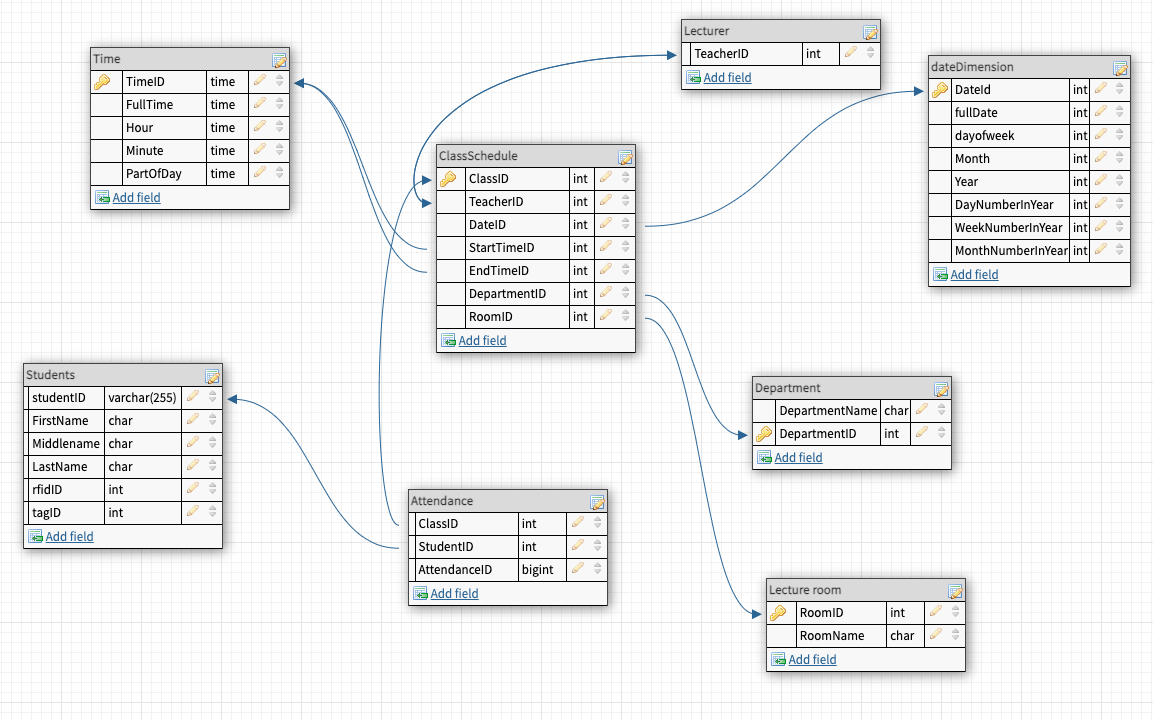
\includegraphics[scale=0.4]{Design & Implementation/images/database_design.png}
  \caption{database design}
\end{figure}

